%----------------------------------------------------------------------------------------
%	PACKAGES AND OTHER DOCUMENT CONFIGURATIONS
%----------------------------------------------------------------------------------------

\documentclass[final,hyperref={pdfpagelabels=false},20pt]{beamer}

% \documentclass[20pt]{beamer}

\usepackage[size=custom,width=76.2,height=106.68,scale=1.2,orientation=portrait]{beamerposter}
% Use the beamerposter package for laying out the poster with a portrait orientation and 30'' by 42'' paper size

\usetheme{I6pd2} 
% Use the I6pd2 theme supplied with this template

\usepackage[english]{babel} 
% English language/hyphenation

\usepackage{amsmath,amsthm,amssymb,latexsym} 
% For including math equations, theorems, symbols, etc

%\usepackage{times}\usefonttheme{professionalfonts}  % Uncomment to use Times as the main font
%\usefonttheme[onlymath]{serif} % Uncomment to use a Serif font within math environments

\boldmath 
% Use bold for everything within the math environment

\usepackage{booktabs} 
% Top and bottom rules for tables

\usepackage{natbib}
% added for bibtex

\graphicspath{{figures/}} 
% Location of the graphics files

\usecaptiontemplate{\small\structure{\insertcaptionname~\insertcaptionnumber: }\insertcaption} 
% A fix for figure numbering

%-------------------------
%      BACKGROUND IMAGE
%-------------------------

\usebackgroundtemplate{
\includegraphics[height=\paperheight, width=\paperwidth]{background}}

%----------------------------------------------------------------------------------------
%	TITLE SECTION 
%----------------------------------------------------------------------------------------

\title{\huge Project Matryoshka: NDN Multiplayer Online Game}
% Title

\author[AuthorNames]{Zhehao Wang\inst{1}, Zening Qu\inst{2}, Jeff Burke\inst{3}}
\institute[Institutes]{\inst{1} \inst{2} \inst{3} UCLA REMAP}

%----------------------------------------------------------------------------------------
%	FOOTER TEXT
%----------------------------------------------------------------------------------------

\newcommand{\leftfoot}{ACM Conference on Information-Centric Networking, Sept 26th, 2014} % Left footer text
\newcommand{\rightfoot}{zhehao.mail@gmail.com} % Right footer text

%----------------------------------------------------------------------------------------
\newcommand{\Csharp}{%
  {\settoheight{\dimen0}{C}C\kern-.05em \resizebox{!}{\dimen0}{\raisebox{\depth}{\#}}}}

\begin{document}

\addtobeamertemplate{block end}{}{\vspace*{2ex}} % White space under blocks

\begin{frame}[t] % The whole poster is enclosed in one beamer frame

\begin{columns}[t] % The whole poster consists of two major columns, each of which can be subdivided further with another \begin{columns} block - the [t] argument aligns each column's content to the top

\begin{column}{.02\textwidth}\end{column} % Empty spacer column

\begin{column}{.465\textwidth} % The first column

%----------------------------------------------------------------------------------------
%	Abstract
%----------------------------------------------------------------------------------------

\begin{block}{Introduction}

Matryoshka is a peer-to-peer multiplayer online game (MOG) running on Named Data Networking (NDN). \newline
We identify the MOG synchronization problem, then propose an octree partition of the game world, and a two-step synchronization design. 
\newline
\begin{itemize}
\item \textbf{Background} 
\end{itemize}
Peer-to-peer structures were explored for online games. \newline
Maintaining security and availability while scaling users has driven most MOGs towards a client-server or client-superpeer architecture.\newline
Client-server games face certain problems: \newline
1. a small number of points of failure; \newline
2. traffic centralizing at servers. \newline
To tackle these problems, we present Matryoshka, whose design is based on Sync: by exchanging data digest each party learns about the missing data, and then can retrieve data via built-in multicast delivery. \newline
The demo demonstrate Matryoshka's gameplay.
\newline
\begin{itemize}
\item \textbf{Gameplay}
\begin{columns}
\begin{column}{.40\textwidth}
\begin{itemize}
\item Play as a matryoshka
\item Explore unknown universe
\item Discover other players
\item Get player position updates
\item Interact with environment
\end{itemize}
\end{column}

\begin{column}{.55\textwidth}
\begin{figure}
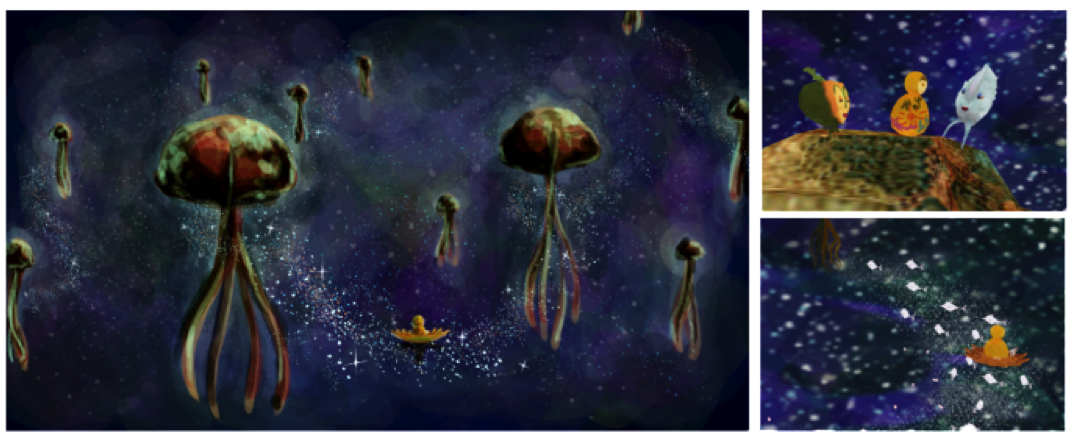
\includegraphics[width=0.9\linewidth]{gamestory}
\caption{Game play}
\label{fig:gamestory}
\end{figure}
\end{column}
\end{columns}

\end{itemize}

\end{block}

%----------------------------------------------------------------------------------------
%	Problem Analysis
%----------------------------------------------------------------------------------------

\begin{block}{Problem Analysis}

The challenge of the MOG: peer-to-peer synchronization in a distributed virtual environment.
\begin{columns}
\begin{column}{.42\textwidth}
\begin{itemize}
\item Synchronization \newline
Players whose areas of interest intersect with each other should reach consistent conclusions about things in the intersected area.
\item Locality \newline
A player needs to know the updates of objects within its Area of Interest (AoI) in the virtual game world.
\end{itemize}
\end{column}

\begin{column}{.52\textwidth}
\begin{figure}
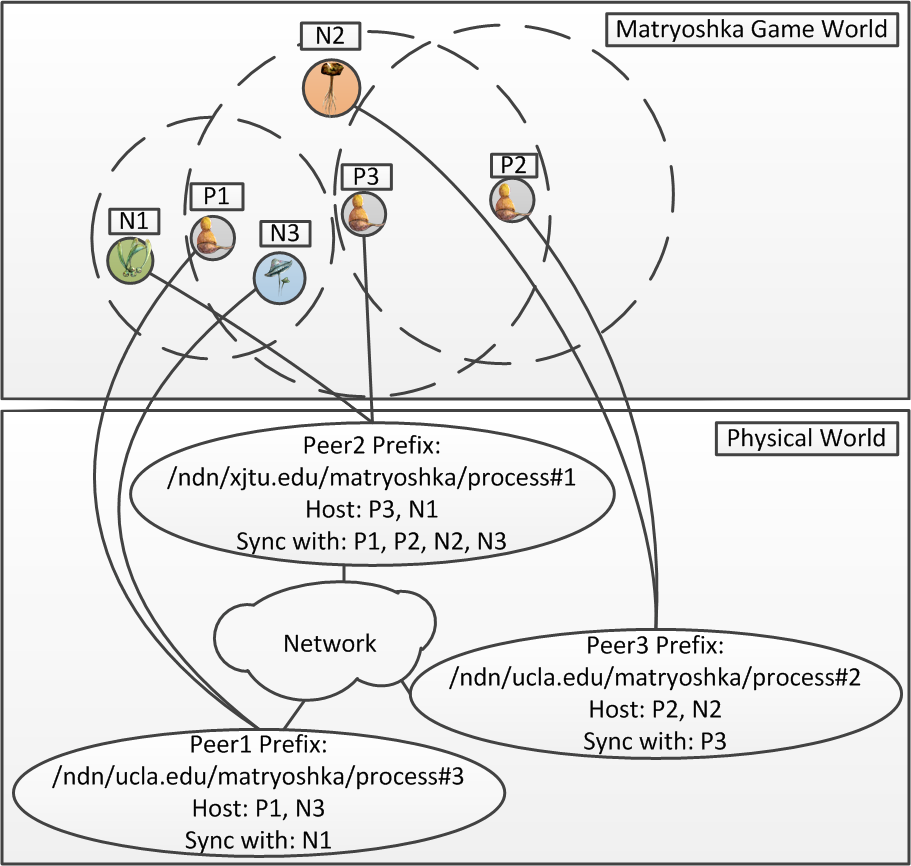
\includegraphics[width=1\linewidth]{ProblemDemo}
\caption{Two worlds in the MOG}
\label{fig:twoworlds}
\end{figure}

\end{column}

\end{columns}

\begin{column}{.01\textwidth}
\end{column}

Figure \ref{fig:twoworlds} illustrates the problem. \newline
Each physical peer hosts a player. Take peer 2 as example.
\begin{itemize}
\item It hosts player3.
\item It should discover player1, player2, NPC2 and NPC3.
\item Its knowledge of player1 and 2's locations should be updated.
\item The AoI should move as player3 moves.
\end{itemize}
\end{block}

%------------------------------------------------
%   Virtual World Partitioning
%------------------------------------------------

\begin{block}{Virtual World Partitioning}

Figure \ref{fig:octrees} illustrates the octree partition of the virtual environment. \newline
The whole world is represented by a top-level cube.
\begin{columns}

\begin{column}{.01\textwidth}
\end{column}

\begin{column}{.50\textwidth}
\begin{itemize}
\item Octree partitions the virtual environment into octants statically and recursively. 
\item With octree, we provide a shared namespace: all the peers that care about the same region can share the data brought by synchronization interests.
\end{itemize}
\end{column}

\begin{column}{.47\textwidth}
\begin{figure}
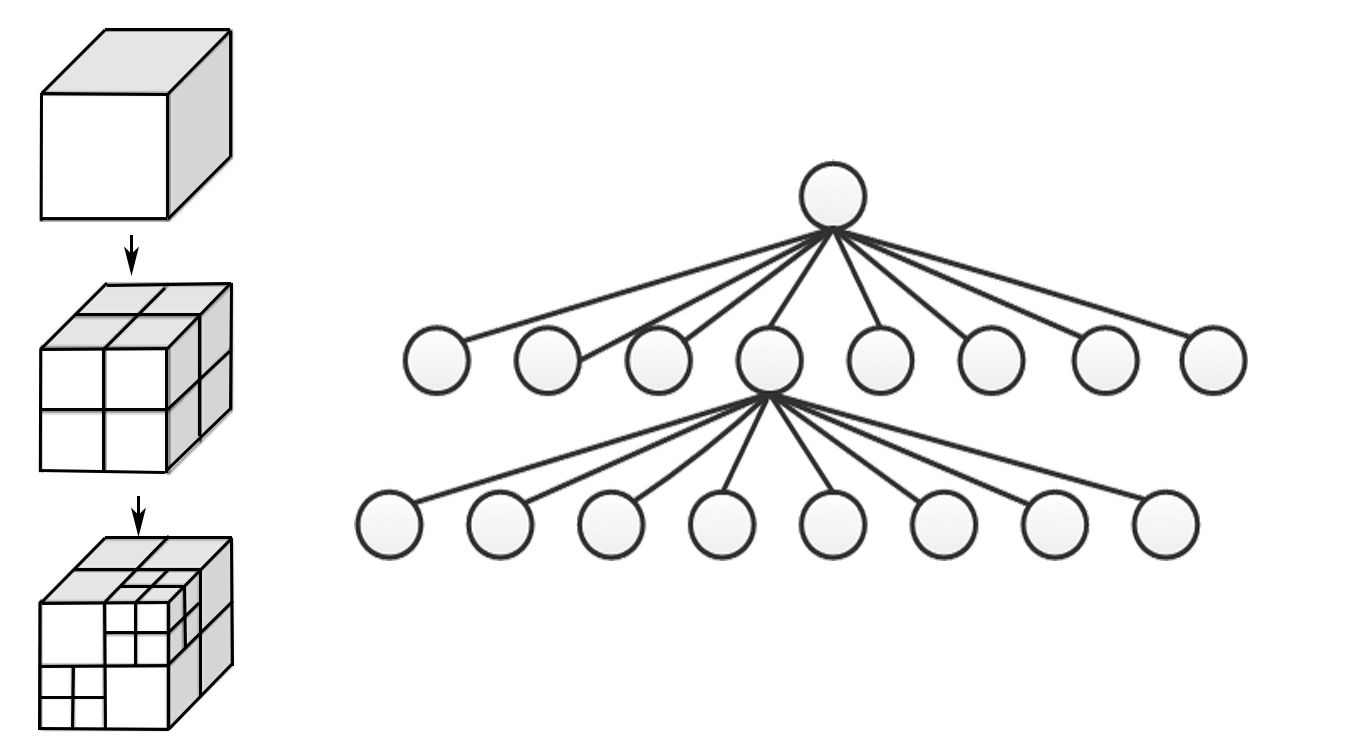
\includegraphics[width=\linewidth]{Octrees}
\caption{Octree partitioning}
\label{fig:octrees}
\end{figure}
\end{column}
\end{columns}

\end{block}

%----------------------------------------------------------------------------------------
%	CONTACT INFORMATION
%----------------------------------------------------------------------------------------

\setbeamercolor{block title}{fg=black,bg=orange!70} % Change the block title color

\begin{block}{Contact Information}

\begin{itemize}
\item Email: \href{mailto:wangzhehao410305@gmail.com}{wangzhehao410305@gmail.com}
\end{itemize}

\end{block}

%-----------------------------------
\end{column} % End of the first column

\begin{column}{.02\textwidth}\end{column} % Empty spacer column
 
\begin{column}{.465\textwidth} % The second column

%----------------------------------------------------------------------------------------
%	Design Overview
%----------------------------------------------------------------------------------------

\begin{block}{Design Overview}

Two-step design:
\begin{itemize}
\item \textbf{Discovery}: which players are in a peer's vicinity. \newline
Peers with overlapping AoIs synchronize "discovery namespaces" for octants of mutual interest to find other objects in the game world:
\begin{itemize}
\item They periodically express Interests in the discovery namespace containing the octant indices they are interested in to all peers, along with a digest of the object names they know in each octant.   
\item Each peer responds with their knowledge of objects in the octants.
\end{itemize}
The namespace for discovery is given in Figure \ref{fig:discoverynamespace}. 
\begin{itemize}
\item Game name component separates the game into sub-worlds.
\item Octant indices indicate the octant’s absolute location in the game world. 
\item Digest component contains the hash of the set of object names.
\end{itemize}
All peers have the same hash for octants belonging to their intersection when steady state is reached.
\end{itemize}

\begin{columns}
\begin{column}{.42\textwidth}

\begin{figure}
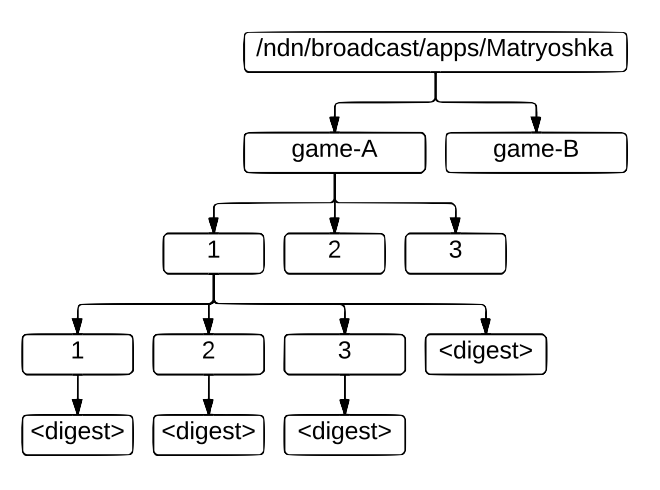
\includegraphics[width=\linewidth]{DiscoveryNamespace}
\caption{Discovery namespace}
\label{fig:discoverynamespace}
\end{figure}
\end{column}

\begin{column}{.54\textwidth}
\begin{figure}
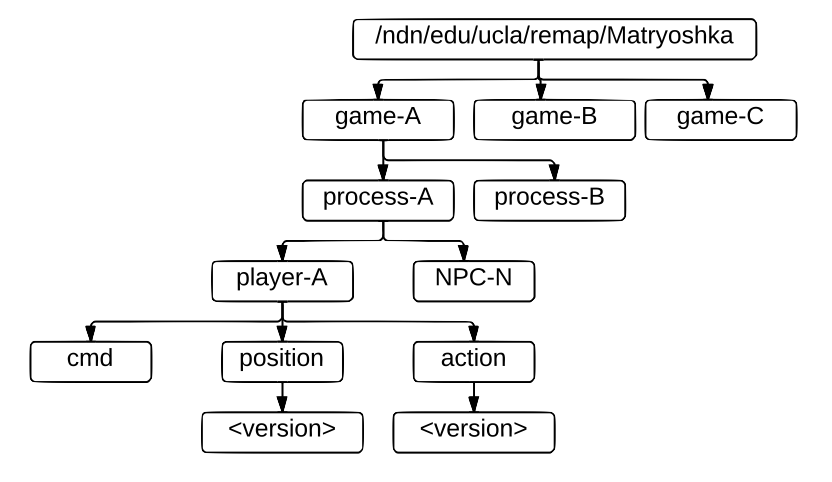
\includegraphics[width=\linewidth]{UpdateNamespace}
\caption{Update namespace}
\label{fig:updatenamespace}
\end{figure}
\end{column}
\end{columns}

\begin{column}{.01\textwidth}
\end{column}

\begin{itemize}
\item \textbf{Update}: what are players doing.
\begin{itemize}
\item Peers express position update interests using the object names returned in step one. 
\item Peers publish their location with sequence numbers.
\end{itemize}
Figure \ref{fig:updatenamespace} illustrates the update namespace.
\begin{itemize}
\item Process name represents a game instance, which hosts the player avatar.
\item Position and action components fetch the latest data.
\end{itemize}
\end{itemize}
Pattern of communication for a game instance (a) to discovery another instance (d) is given in Figure \ref{fig:samplenames}.
\begin{figure}
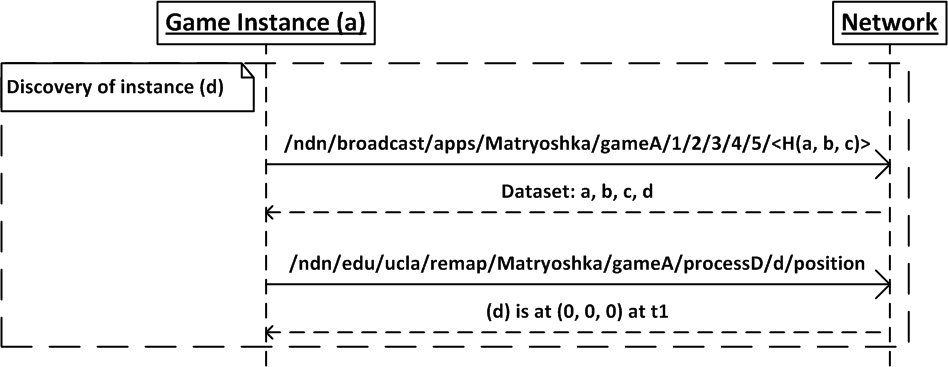
\includegraphics[width=0.66\linewidth]{SampleNames}
\caption{Example names}
\label{fig:samplenames}
\end{figure}

\end{block}

%----------------------------------------------------------------------------------------
%	Demo Implementation
%----------------------------------------------------------------------------------------

\begin{block}{Demo Implementation}

\begin{column}{.01\textwidth}
\end{column}

The demo application was built using Unity3D game engine, and ndn-dot-net, a \Csharp{} adaptation of NDN Common Client Library. The demo shows the game code running on a small number of peers, and a visualization of the AoI. \newline
Player characters and NPCs are instantiated by each peer, and each peer can navigate around the common world using their player character. Player and NPC discovery, and player position update (at a rate of 25 Hz) is demonstrated.
\newline
\end{block}

%----------------------------------------------------------------------------------------
%	Conclusion & Future Work
%----------------------------------------------------------------------------------------

\begin{block}{Future Work}
Future work includes further evaluation of the design, and addressing problems caused by hierarchical octree partitioning.
\begin{itemize}
\item Difficult to represent AoIs that are close to the border between two sub-regions of the highest subdivision hierarchy.
\item Difficult to represent spherical AoI.
\item Need routing to keep up with the changes in AoI represented by octree.
\end{itemize}
\end{block}

%----------------------------------------------------------------------------------------
%	REFERENCES
%----------------------------------------------------------------------------------------

\begin{block}{References}
        
\nocite{*}
% Insert publications even if they are not cited in the poster
\small{\bibliographystyle{unsrt}
\bibliography{reference}}

\end{block}

%----------------------------------------------------------------------------------------

\end{column} % End of the second column

\begin{column}{.015\textwidth}\end{column} % Empty spacer column

\end{columns} % End of all the columns in the poster

\end{frame} % End of the enclosing frame

\end{document}